\chapter{Introduction}\label{ch:introduction}
In most laboratories around the world, computers are in charge of controlling experiments. From complex systems such as particle accelerators to simpler UV-Vis spectrometers, there is always a computer responsible for asking the user for some input, performing a measurement, and displaying the results. Learning how to control devices through the computer is, therefore, of the utmost importance for every experimentalist who wants to gain a deeper degree of freedom when planning measurements.

This book is task-oriented, meaning that it focusses on how things can be done and not on much theory on how programming works in general. This approach can lead to some generalizations that may not be correct in all scenarios. I ask your forgiveness in those cases and your cooperation: if you find anything that can be improved or corrected, please contact me.

Together with the book, there is a website\footnote{https://www.pythonforthelab.com} where you can find extra information, anecdotes, and examples that didn't fit in here. Remember that the website and its forum are the proper places to communicate with fellow Python For The Lab readers. If you are stuck with the exercises or you have questions that we don't answer in the book, don't hesitate to shout in the forum. Continuous feedback is the best way to improve this book.

\section{What are you going to learn}\label{sec:what-are-you-going-to-learn}
\begin{center}
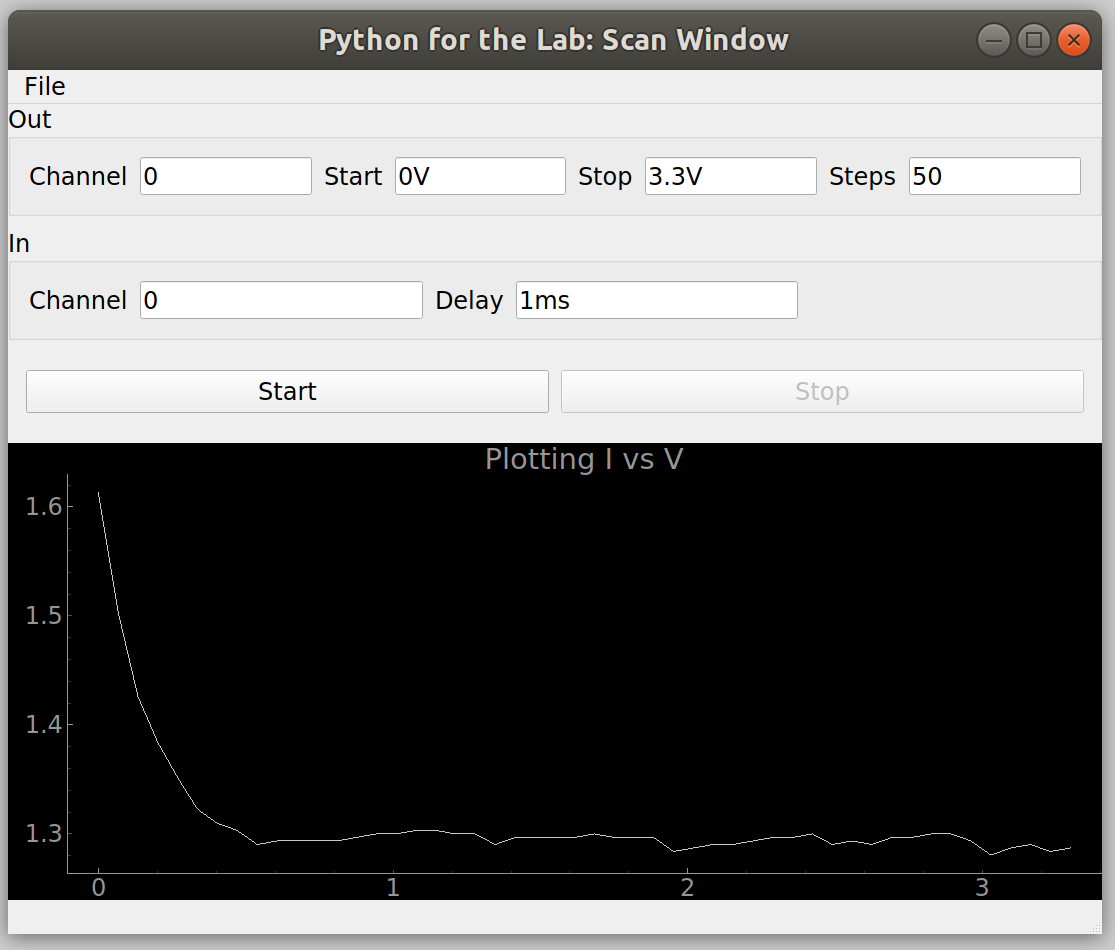
\includegraphics[width=.6\linewidth]{images/Chapter_01/screenshot.png}
\end{center}

This book is the result of many years developing software for scientific applications and, more importantly, of several workshops organized in different universities and companies around Europe. In this time, we have gained experience developing new programs, and we have also collected invaluable feedback from students. With these two elements, we have designed the book in a way that allows the reader to improve their Python proficiency at the same time that we show a clear path to get started with instrumentation software.

Each chapter was carefully crafted to introduce new Python topics next to specific tools needed to control an experiment. For example, in Chapter~\ref{ch:first-driver}, we develop a driver for a device and take a first dive into classes and objects. We introduce threads in Chapter~\ref{ch:run-experiment} when we discuss how to be able to stop a running experiment. We also cover how to create user interfaces to accept user input and display data in real-time, such as in the image above. We believe that by following a task-oriented approach, students get the initial direction, tools, and vocabulary to ask for help if needed.

Regarding instrumentation itself, we have compiled what we believe are best practices that speed up the development of solutions and ensure a more prolonged survival of the programs. We discuss how to follow programming patterns that allow the exchange of solutions between people from the same lab or from across the world. This book is not a programmer's book, but a scientist's book written for another scientist. We try to use clear and concise language as much as possible, avoiding jargon when not necessary.

\section{Who Can Read this Book}\label{sec:who-can-read-this-book}
To follow the book, we don't assume proficiency in Python. We only require people to have a grasp of \textit{if-statements}, \textit{for-loops}, and \textit{while-loops}, and when to use them. We build the knowledge when it is required, through carefully crafted examples and exercises. If the reader is already proficient in Python, we believe there is value in the best practices we show, in how we structure the code, and how we decided to solve problems. The path is never one, but the goal is the same: extend the possibilities of an experiment by controlling it with custom software.

We believe that anybody working in a lab already has some knowledge of how to perform an experiment. The book proposes to measure the I-V curve of a diode. It is not required to understand the phenomenon, we simply use it as an example of an experiment in which a voltage is varied, and another voltage is measured. This simple example is the building block of most experiments, from controlling temperatures to moving piezo-stages, to tuning the frequency of a laser. By using an LED as the diode in the experiment, we can literally see the effect of applying a voltage.

\section{Why building your software}\label{sec:why-building-your-software}
Computers and the software within them, should be regarded as tools and not as obstacles in a researcher's daily tasks. However, when it comes to controlling a setup, many scientists prefer to be bound by the specifications of the software provided instead of pursuing innovative ideas. Once a researcher learns how to develop their programs, these limits fall, and creativity can sprout. With automation, the throughput of the setup can increase, human errors can be reduced, or experiments that were no possible become reachable through the introduction of feedback loops.

However, there is an added consideration while building software for research labs: reproducibility. It is a primary concern for modern scientists on how to be able to reproduce results and how to enable others to perform the same measurements. We believe that open-sourcing software as much as possible lowers the entry barrier, and allows present and future colleagues to build on experience instead of reinventing it. The practices we follow in the book are ideal for sharing entire programs or at least parts of them with the community.

\section{PFTL DAQ Device}\label{sec:pftl-daq-device}
We have developed a device nicknamed {PFTL DAQ} that works as a data acquisition board. The instructor provides these boards during the workshops, but if you got this book online and would like to buy one of PFTL DAQ's, please contact us\footnote{courses@pythonforthelab.com}. The devices are open source/open hardware, they are based on the Arduino DUE, and you can find the instructions for building one on our website. If you have access to any other acquisition card, with a bit of tinkering, you will be able to adapt the course contents to your needs.

Building software for the lab has a reality component not covered in any other books or tutorials. The fact that we are interacting with real-world devices, which can change the state of an experiment, makes the development process much more compelling. The PFTL DAQ is a toy device, easy to replace, but capable of performing quantitative measurements.

\section{Why Python?}\label{sec:why-python?}
Python became ubiquitous in many research labs because of many different reasons. First, Python is open source, and we firmly believe that the future of research lies in openness. Even for an industrial researcher, the results and the process for generating data should be open to your colleagues (present and future). Python leverages the knowledge gathered in very different areas to deliver a better product. From high-performance computing to machine learning, to experiments, to websites, Python can be found everywhere.

Another factor to take into account is that Python is free, and therefore there is no overhead when implementing it. There are no limits to the number of machines in which you can install Python, nor the number of different simultaneous users. Moreover, there is a myriad of professionally developed tools such as numpy, scipy, scikit. Companies such as Anaconda provide customers with high-quality advice and troubleshooting, feeling an often encountered gap with open-source software.

However, for experimentalists, there is a big downside when considering Python. Searching online for instructions on how to control an experiment, few sources appear and even less if focusing on Python alone. Fortunately, this is changing thanks to an evergrowing number of people developing open source code and writing handy documentation. Python can achieve all the same functionality of LabView. The only limitation is the existence of drivers for more sophisticated instruments. With a stronger community, companies will realize the value of providing those drivers for other programming environments.

But the choice of Python is not restricted to the lab. In many cases, Python is used for data analysis, and therefore it makes sense to bring its use to the source of the data: the experiment itself. Moreover, with Python, it is possible to build websites, develop machine learning algorithms, automatize your daily tasks, and many more exciting things. Learning Python increases the employability chances in and out of academia, both for people wishing to continue working with experiments or for people who want to focus on data analysis or beyond.

\section{The Onion Principle}\label{sec:onion-principle}
When we start developing software, it is tough to think ahead. Most likely, we have a small problem that we want to solve as quickly as possible, and we just go for it. Later on, it may turn out that the small problem is something worth investigating deeper. Our software will not be able to handle the new tasks, and we will need to improve it. Having a proper set of rules in place will help us develop code that can adapt to our future needs while keeping us productive in the present. We like to call those rules the Onion Principle.

The rules we are talking about are not rules written in stone. They are not found in books (by the way, they are not here either). We are talking about a state of mind that empowers ourselves to develop better, clearer, and more expandable code. Sitting down and reflecting is the best we can do, even more than sitting down and typing. When dealing with experiments, we have many things to ask ourselves, what do we know, what do we want to prove how to do it. Only then will we sit down to write a program that responds to our needs.

If we build something that we cannot expand, it becomes useless very soon. When we don't know what may happen with our code, we should think ahead and structure it as an onion, in layers. It is not something that happens naturally, but we can develop our set of procedures to ensure that we are developing future-proof code. Once we get the handle on it, it won't take us longer than being disorganized and not having the proper structure. We can avoid variables that are not self-descriptive, lack of comments, and the list goes on and on.

It is not all about being future-proof. When we start with a simple task at hand, we want to solve it quickly and not to spend hours developing useless lines of code just thinking what if. It is also known as premature optimization. If we spend much time trying to solve a problem that may appear, we might just not see the problem that will arise. Therefore, it is better to fail quickly and improve than to fail later and run out of time. However, having a strong foundation is always important. Taking shortcuts just because we don't want to create a separate file will give us more headaches, even in the short term. We should build code that is robust enough to support for expansion later on. In the same way that we take several steps to perform an experiment, starting with the sample preparation, we should take steps when developing software.

In this book, we go from the one-off script that can get the job done in a matter of minutes, to a fully-fledged user interface that allows us to change the parameters of the experiment and visualize them in real-time.

\section{Where to get the code}\label{sec:where-to-get-the-code}
The code that we develop through the book is freely available on Github\footnote{https://github.com/PFTL}. The code is organized by chapters, to make it more accessible while reading. There is also an extra folder with a version of the program that goes beyond what the book covers. For example, the code includes documentation and an installation script. In this way, the readers can have an idea of the possible directions to take for their software.

If you have found any errors or would like to contact us, please send an e-mail to courses@pythonforthelab.com. We will come back to you as soon as possible.

\section{Organizing a Python for the Lab Workshop}\label{sec:organizing-a-python-for-the-lab-workshop}
Python for the Lab was born to bring together researchers working in a lab and the Python programming language. With that goal in mind, we developed not only this book but also a workshop in which we can train scientists. The workshops change in duration and content, and we can adapt them to the specific needs of the group.

If you would like to organize a Python for the Lab workshop at your institution, contact us at courses@pythonforthelab.com, and we will gladly discuss with you the different options. You can also find more information about the courses at https://www.pythonforthelab.com.
